\appendix
\chapter{Learning discourse structure: Unsupervised}
\label{app:latent}

\begin{table*}[t]
\centering
\small
\begin{tabular}{lllllll}
\toprule
                    &         & \multicolumn{4}{c}{Number of documents}  &             \\ \cline{3-6}
Dataset             & Classes & Total & Train & Dev & Test    & Vocab. \\ 
\midrule
Yelp           & 5       & 333K  & 266,522  & 33,333  & 33,317 & 53K        \\
Debates & 2       & 1.5K  & 1,050    & 102 & 374 & 21K        \\
WQ     & 2       & 7.7K  & 6,195    & 775   & 763     & 150K       \\
WQTC     & 2       & 7.8K  & 6,241    & 777         & 794     & 131K       \\
WSJSO     & -       &2.4K    & 1,950 (35,165)         & 247 (4,392)    & 241 (4,383) &49K\\ \bottomrule
\end{tabular}
\vspace{-0.4em}
\caption{Statistics for the datasets used in the text classification and discrimination tasks (calculated after preprocessing). For WSJSO, the number of generated pairs are in parentheses.}
\label{tab:corpora}
\end{table*}
\section{Datasets} Statistics for the datasets are listed in Table \ref{tab:corpora}. 

\begin{table*}[t]
\small
\centering
\renewcommand{\tabcolsep}{1.3mm}
\begin{tabular}{llllll}
\toprule
                    & Yelp & Debates & WQ & WQTC & WSJSO  \\
\midrule
tree height     & 2.049 (2.248) &2.751 (2.444)&2.909 (2.300) &4.035 (2.468) &2.288 (2.368)\\
prop. of leaf nodes  & 0.825 (0.801) & 0.849 (0.869) &0.958 (0.971) &0.931 (0.966) &0.892 (0.888)\\
%parent entropy & 0.456 &0.600 &0.455 &0.774   &0.474  \\
norm. arc length & 0.433 (0.468) &	0.397 (0.377) & 0.420 (0.377) & 0.396 (0.391)	&0.426 (0.374)\\
\% vacuous trees & 73\% (68\%) &38\% (40\%) &42\% (28\%) &14\% (21\%) &100\% (56\%)\\
\bottomrule
\end{tabular}
\vspace{-0.4em}
\caption{Statistics for the learned trees averaged across four runs on the L\&L(ours) model with comparisons (in parentheses) to results using the original L\&L code without the design change or bug fix.}
\label{tab:trees_full_orig}
\vspace{-0.7em}
\end{table*}

\begin{table*}[t]
\centering
\small
\scalebox{0.9}{
\begin{tabular}{p{2.2cm} l p{0.8cm} p{0.85cm} p{0.8cm} p{1.2cm} p{0.8cm}}
\toprule
 & Accuracy & tree height & prop. of leaf & parent entr. & norm. arc length & \%vac. trees \\
\midrule
Full           & 82.49\thinspace$|$\thinspace\textbf{81.11} (0.95) & 4.035 & 0.931 &0.774 &0.396 &14\%\\
-biLSTM & 80.35\thinspace$|$\thinspace\ 77.80 (1.72) & 11.51 & 0.769 &1.876 &0.353 &4\%\\
-biLSTM, +p & 78.72\thinspace$|$\thinspace\ 77.11 (2.18) &10.430 &0.790 &0.349 &0.349 &3\% \\
-biLSTM, +4p & 82.75\thinspace$|$\thinspace\ \textbf{81.71} (0.70) & 9.588 & 0.811 &1.60 & 0.353 & 3\% \\
-biLSTM, +w & 78.46\thinspace$|$\thinspace\ 75.57 (2.52) &7.364 &0.856 &1.307 &0.359 & 3\% \\
-biLSTM, +w, +p & 77.08\thinspace$|$\thinspace\ 74.78 (2.58) &8.747 & 0.826 & 1.519 &0.349 &4\%\\
\midrule
parsed RST &- &25.084 &0.567 & 2.711 &0.063 &0\%\\
\bottomrule
\end{tabular}}
\caption{Max\thinspace$|$ mean (standard deviation) test accuracy and tree statistics of the WQTC dev set (averaged across four training runs with different initialization weights). Bolded numbers are within 1 standard deviation of the best performing model. +w uses the weighted sum, +p adds 1 extra level of percolation, +4p adds 4 levels of percolation. The last row are the (`gold') parsed RST discourse dependency trees.}
\label{tab:results_deeper_detail}
\end{table*}

For WQ, the `very good' class was created by \citet{Louis:2013} using as a seed the 63 articles in the New York Times corpus \cite{Sandhaus:2008} deemed to be high-quality writing by a team of expert journalists. The class was then expanded by adding all other science articles in the NYT corpus that were written by the seed authors (4,253 articles). For the ‘typical’ class, science articles by all other authors were included (19,520). Because the data is very imbalanced, we undersample the ‘typical’ class to be the same size as the ‘very good’. We split this data into 80/10/10 for training, development and test, with both classes equally represented in each partition. 

For WQTC, the original dataset authors provide a list of the 10 most topically similar articles for each article.\footnote{\url{http://www.cis.upenn.edu/~nlp/corpora/scinewscorpus.html}} We make use of this list to explicitly sample topically similar documents.

\section{Preprocessing} For Debates and Yelp, we follow the same preprocessing steps as in L\&L, but do not set a minimum frequency threshold when creating the word embeddings. 
For our three datasets, sentences are split and tokenized using Stanford Core NLP.

\section{Training} For all models, we use the Adagrad optimizer with a learning rate of 0.05. For WQ, WQTC, and WSJSO, gradient clipping is performed using the global norm with a ratio of 1.0. The batch size is 32 for all models except WSJSO uses 16. All models are trained for a maximum of 8 hours on a GeForce GTX 1080 Ti card.

\section{Results}  Because our results hinge on multiple runs of experiments each initialized with different random weights, we include here more detailed versions of our results to more accurately illustrate their variability. Table \ref{tab:trees_full_orig} supplements Table \ref{tab:trees_full} with tree statistics from L\&L(orig), the model \emph{without} the design change or bug fix, to illustrate the derived trees on this model are similar. Finally, Table \ref{tab:results_deeper_detail} is a more detailed version of Table \ref{tab:results_deeper}, which additionally includes  maximum accuracy, standard deviation for accuracy, as well as the average parent entropy calculated over the latent trees. 

\chapter{Subjective discourse}
\label{app:subjective}

\section{Dataset Statement}
\label{sec:app_subjective}

\# Data Statement for SubjectiveResponses

Data set name: SubjectiveResponses

Citation (if available): TBD

Data set developer(s): Elisa Ferracane

Data statement author(s): Elisa Ferracane

Others who contributed to this document: N/A

\#\# A. CURATION RATIONALE 

The purpose of this dataset is to capture subjective judgments of responses to questions. We choose witness testimonials in U.S. congressional hearings because they contain question-answer sessions, are often controversial and elicit subjectivity from untrained crowdsourced workers. The data is sourced from publicly available transcripts provided by the U.S. government (https://www.govinfo.gov/app/collection/chrg) and downloaded using their provided APIs (https://api.govinfo.gov/docs/). We download all transcripts from 113th-116th congresses (available as of September 18, 2019), then use regexes to identify speakers, turns, and turns containing questions. We retain hearings with only one witness and with more than 100 question-response pairs as a signal of argumentativeness. To ensure a variety of topics and political leanings, we sample hearings from each congress and eliminate those whose topic is too unfamiliar to an average American citizen (e.g. discussing a task force in the Nuclear Regulatory Commission). This process yields a total of 20 hearings: 4 hearings from the 113th congress (CHRG-113hhrg86195, CHRG-113hhrg88494, CHRG-113hhrg89598 CHRG-113hhrg93834), 5 hearings from the 114th (CHRG-114hhrg20722, CHRG-114hhrg22125, CHRG-114hhrg26003, CHRG-114hhrg95063, CHRG-114hhrg97630), 7 hearings from the 115th (CHRG-115hhrg25545, CHRG-115hhrg30242, CHRG-115hhrg30956, CHRG-115hhrg31349, CHRG-115hhrg31417, CHRG-115hhrg31504,  CHRG-115hhrg32380), and 4 hearings from the 116th (CHRG-116hhrg35230, CHRG-116hhrg35589, CHRG-116hhrg36001, CHRG-116hhrg37282). For annotation, we then select the first 50 question-response pairs from each hearing.

The dataset and code used to create the dataset is available at \url{http://github.com/elisaF/subjective_discourse}.

\#\# B. LANGUAGE VARIETY/VARIETIES

* BCP-47 language tag: en-US

* Language variety description: American English as spoken in U.S. governmental setting

\#\# C. SPEAKER DEMOGRAPHIC

* Description: The speakers are from two groups: the questioners are politicians (members of Congress) and the witnesses can be politicians, businesspeople or other members of the general public. 

* Age: No specific information was collected about the ages, but all are presumed to be adults (30+ years old).

* Gender: No specific information was collected about gender, but members of Congress include both men and women. The witnesses included both men and women.

* Race/ethnicity (according to locally appropriate categories): No information was collected.

* First language(s): No information was collected.

* Socioeconomic status: No information was collected.

* Number of different speakers represented: 91 members of Congress and 20 witnesses.

* Presence of disordered speech: No information was collected but none is expected.
 
\#\# D. ANNOTATOR DEMOGRAPHIC

Annotators:

* Description: Workers on the Amazon Mechanical Turk platform who reported to live in the U.S. and had a $>$95\% approval rating with $>$500 approved HITs were recruited during the time period of November 2019 - March 2020.

* Age: No information was collected.

* Gender: No information was collected.

* Race/ethnicity (according to locally appropriate categories): No information was collected.

* First language(s): No information was collected.

* Training in linguistics/other relevant discipline: None.

Annotation guideline developer:

* Description: The author of this data statement.

* Age: 40.

* Gender: Female.

* Race/ethnicity (according to locally appropriate categories): Hispanic.

* First language(s): American English.

* Training in linguistics/other relevant discipline: PhD in computational linguistics.


\#\# E. SPEECH SITUATION

* Description: Witness testimonials in U.S. congressional hearings spanning the 114th-116th Congresses.

* Time: 2013-2019

* Place: U.S. Congress

* Modality (spoken/signed, written): transcribed from spoken.

* Scripted/edited vs. spontaneous: mostly spontaneous, though members of Congress sometimes read questions they have written down

* Synchronous vs. asynchronous interaction: synchronous

* Intended audience:  the U.S. government and the general public, as all hearings are both transcribed and televised

\#\# F. TEXT CHARACTERISTICS

The genre is political discourse in a highly structured setting where a chairperson runs the meeting, and each member of Congress is afforded 5 minutes to question the witness but can yield their time to others. Topics vary based on the congressional committee that is holding the hearing, and include oversight of other governmental bodies (e.g., IRS, Department of Justice) and inquiries into businesses suspected of misconduct (e.g., FaceBook, Wells Fargo).

\#\# G. RECORDING QUALITY

N/A

\#\# H. OTHER

N/A

\#\# I. PROVENANCE APPENDIX

N/A

\#\# About this document

A data statement is a characterization of a dataset that provides context to allow developers and users to better understand how experimental results might generalize, how software might be appropriately deployed, and what biases might be reflected in systems built on the software.

Data Statements are from the University of Washington. Contact: [datastatements@uw.edu](mailto:datastatements@uw.edu). This document template is licensed as [CC0](https://creativecommons.org/share-your-work/public-domain/cc0/).

This version of the markdown Data Statement is from June 4th 2020. The Data Statement template is based on worksheets distributed at the [2020 LREC workshop on Data Statements](https://sites.google.com/uw.edu/data-statements-for-nlp/), by Emily M. Bender, Batya Friedman, and Angelina McMillan-Major. Adapted to community Markdown template by Leon Dercyznski.

\section{Annotation task}
\label{sec:app_anno}

For each HIT, we provide the hearing title, date and summary, along with titles of the politicians and witness. If there are intervening turns in the conversation that are not part of a question-response pair, we give the annotator the option to view the immediately preceding or following turn (e.g., see `Show/Hide Next Turn' in Figure \ref{fig:subj_amt_screenshots_main}). Each HIT takes an average of 15 minutes to complete. To minimize context switching for annotators and roughly preserve the original conversation order, we publish only a small batch from one hearing at a time, waiting until it completes before publishing the sequentially next one or starting a new hearing.

For judging the response, we first ask the annotator to judge how the witness responds to the question: answers the question, partially answers, shifts the question, or says they can't answer (where a partial answer is a special case of a shifted question that annotators found more intuitive to evaluate separately). Second, we ask the annotator to judge the intent of the witness as being sincere or not.\footnote{For partial answer and can't answer, we also ask whether the witness provides extra information, and if so, whether their intent was sincere or not. However, we ended up discarding the overanswer label in these cases because it was too sparse and noisy to be informative.} Combining the answers from these questions then produces the 6 labels at the bottom tier of Figure \ref{fig:response_taxonomy}. 

During our qualification process, an annotator is rejected based on a combination of the following criteria (ranked in order of importance):
\begin{enumerate}[label=(\roman*)]
\item bad explanations: The explanations are non-sensical (copying random parts of the question or response, or using computer-generated text), incomplete (too short and not explaining the intent), or incongruous (explaining a sincere intent when the label chosen was insincere).
\item bad labels for example items: For examples discussed in the instructions, the functional portion of the label does not match the label in the instructions. 
\item bad labels for unambiguous items: For cases where the functional label is unambiguous (e.g., `Yes' can only be construed as an answer), the label does not match the unambiguous one. 
\item short response times: The annotator response time is shorter than the reading time, as measured by my own time to read all questions and responses without including any time for reasoning about the labels.
\end{enumerate} 

\begin{figure}
\centering
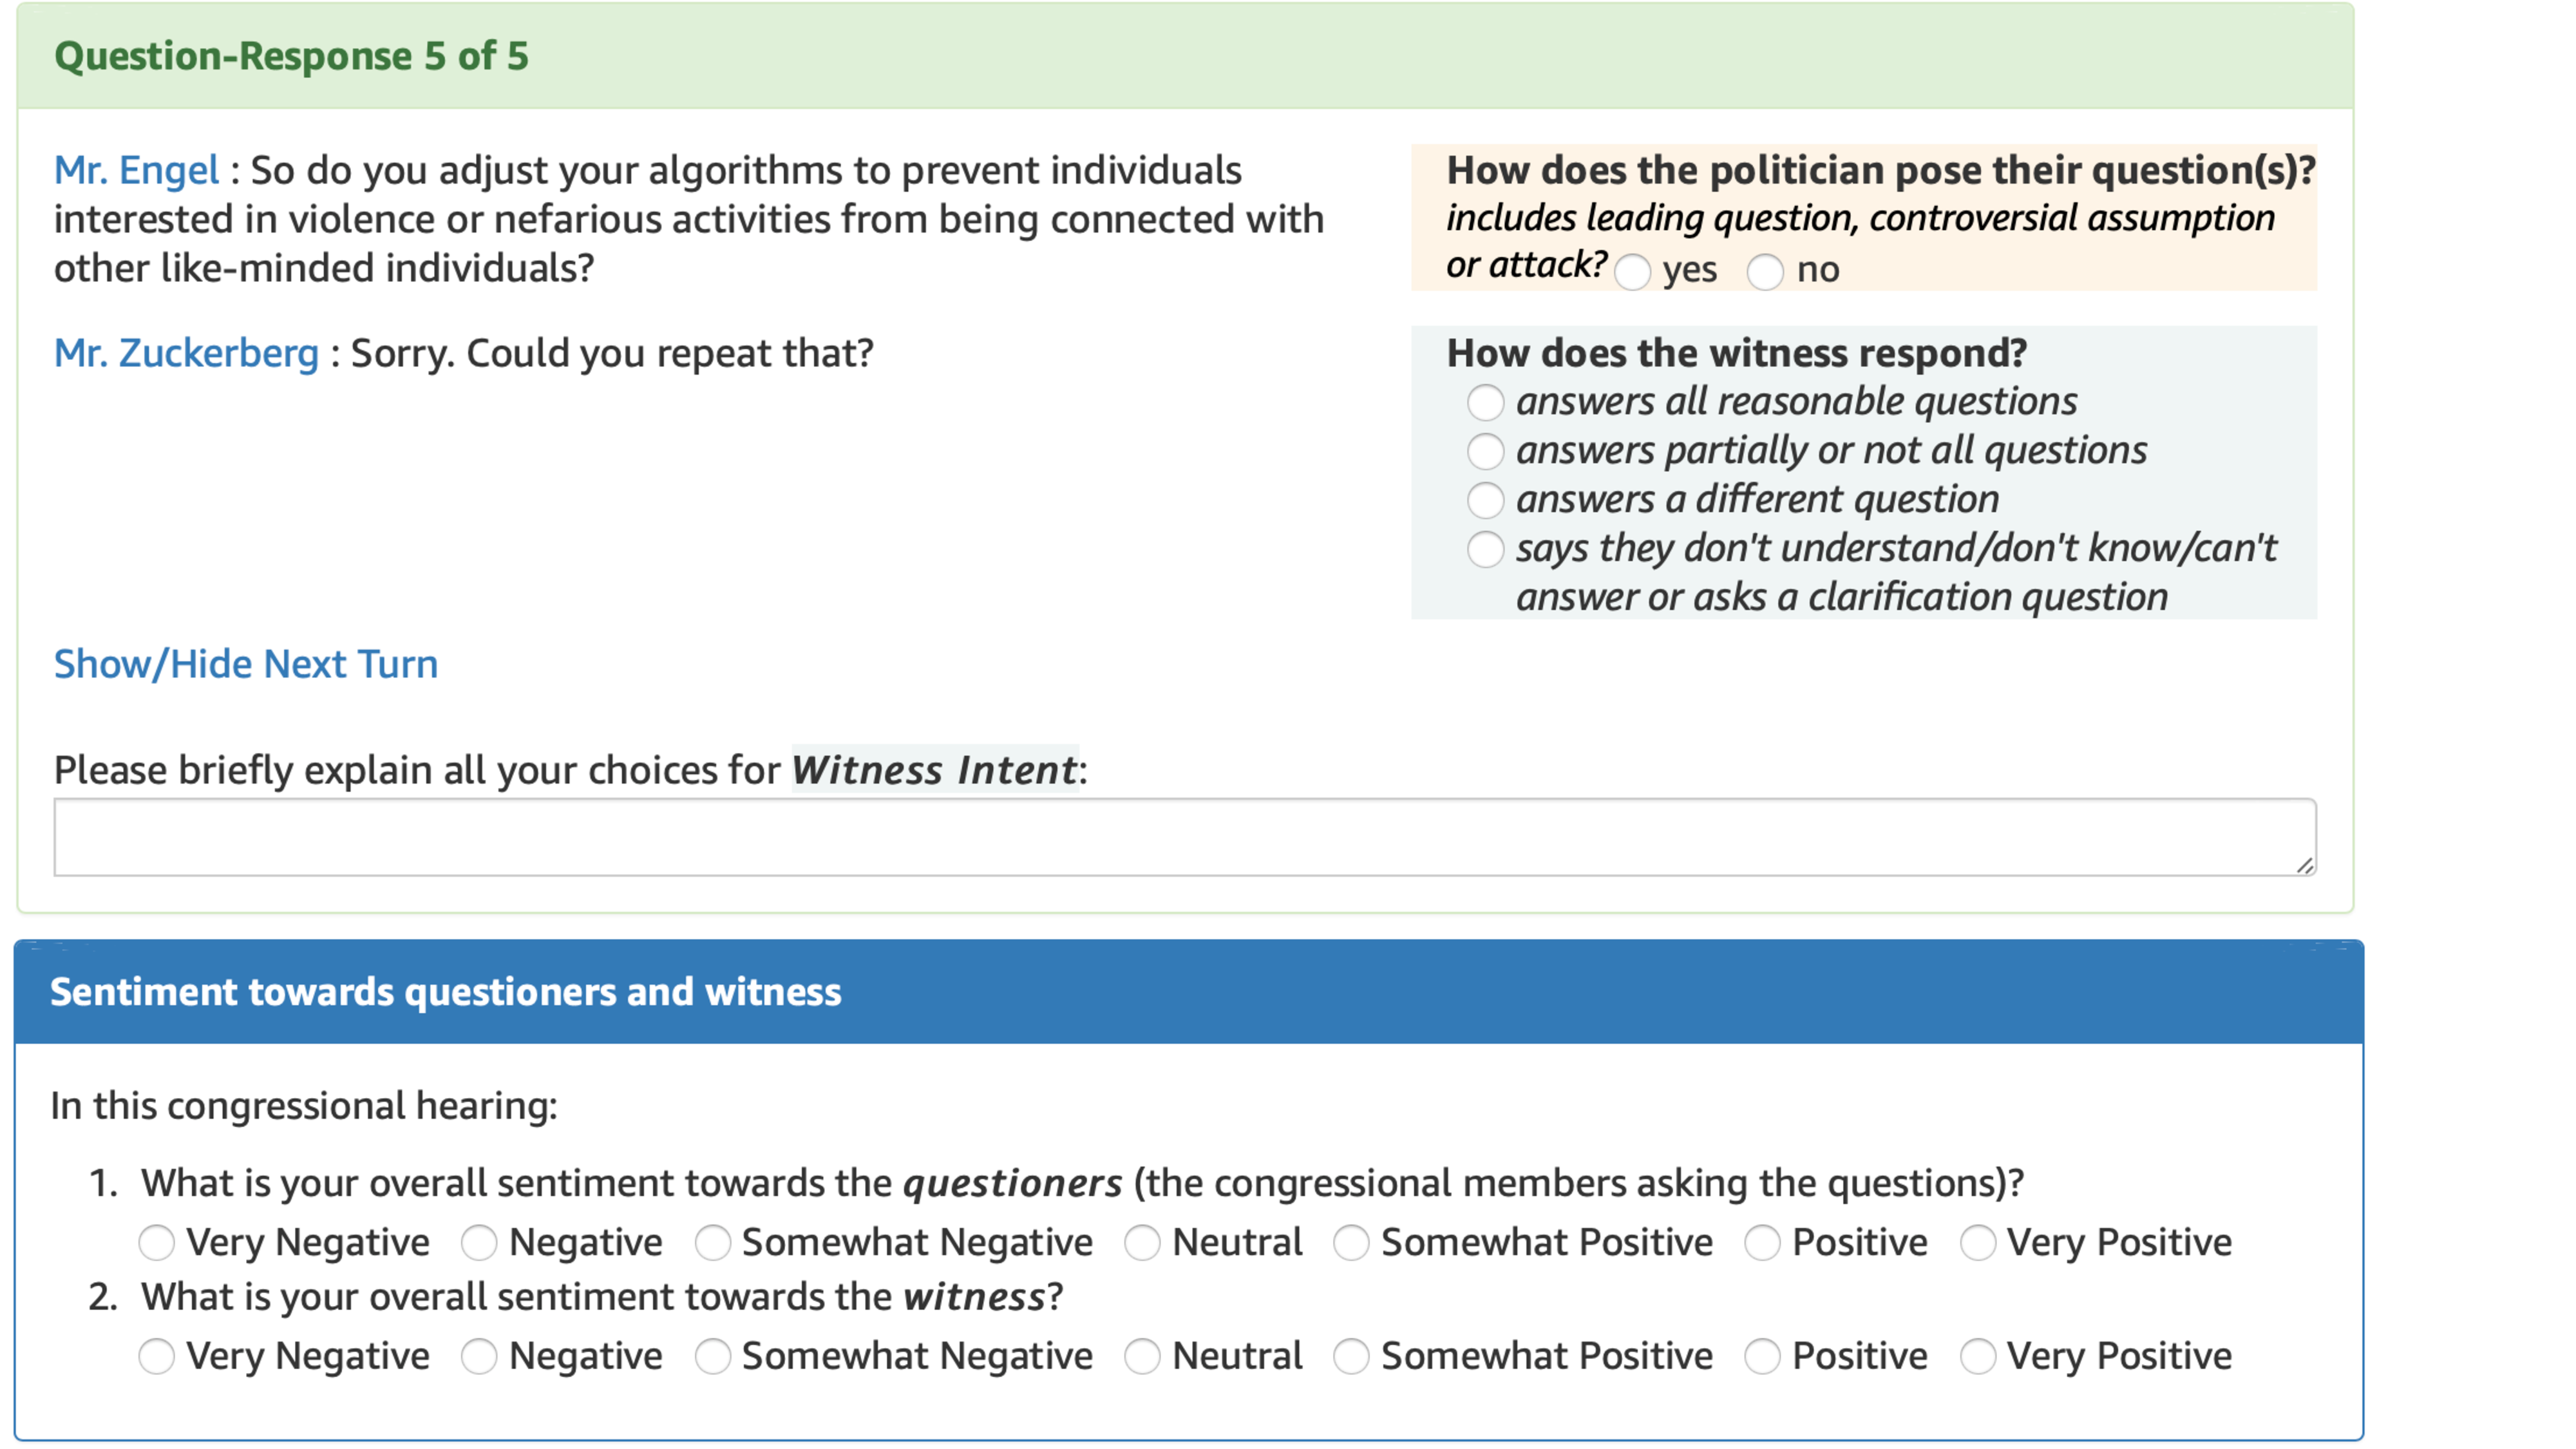
\includegraphics[width=0.99\textwidth]{plots/subj_amt_screenshots_main.pdf}
\vspace{-.3em}
\caption{Overview of the crowdsourced task (only 1 of 5 question-response pairs shown for space).}
\label{fig:subj_amt_screenshots_main}
\end{figure}

\begin{figure}
\centering
\begin{subfigure}{.45\textwidth}
  \centering
  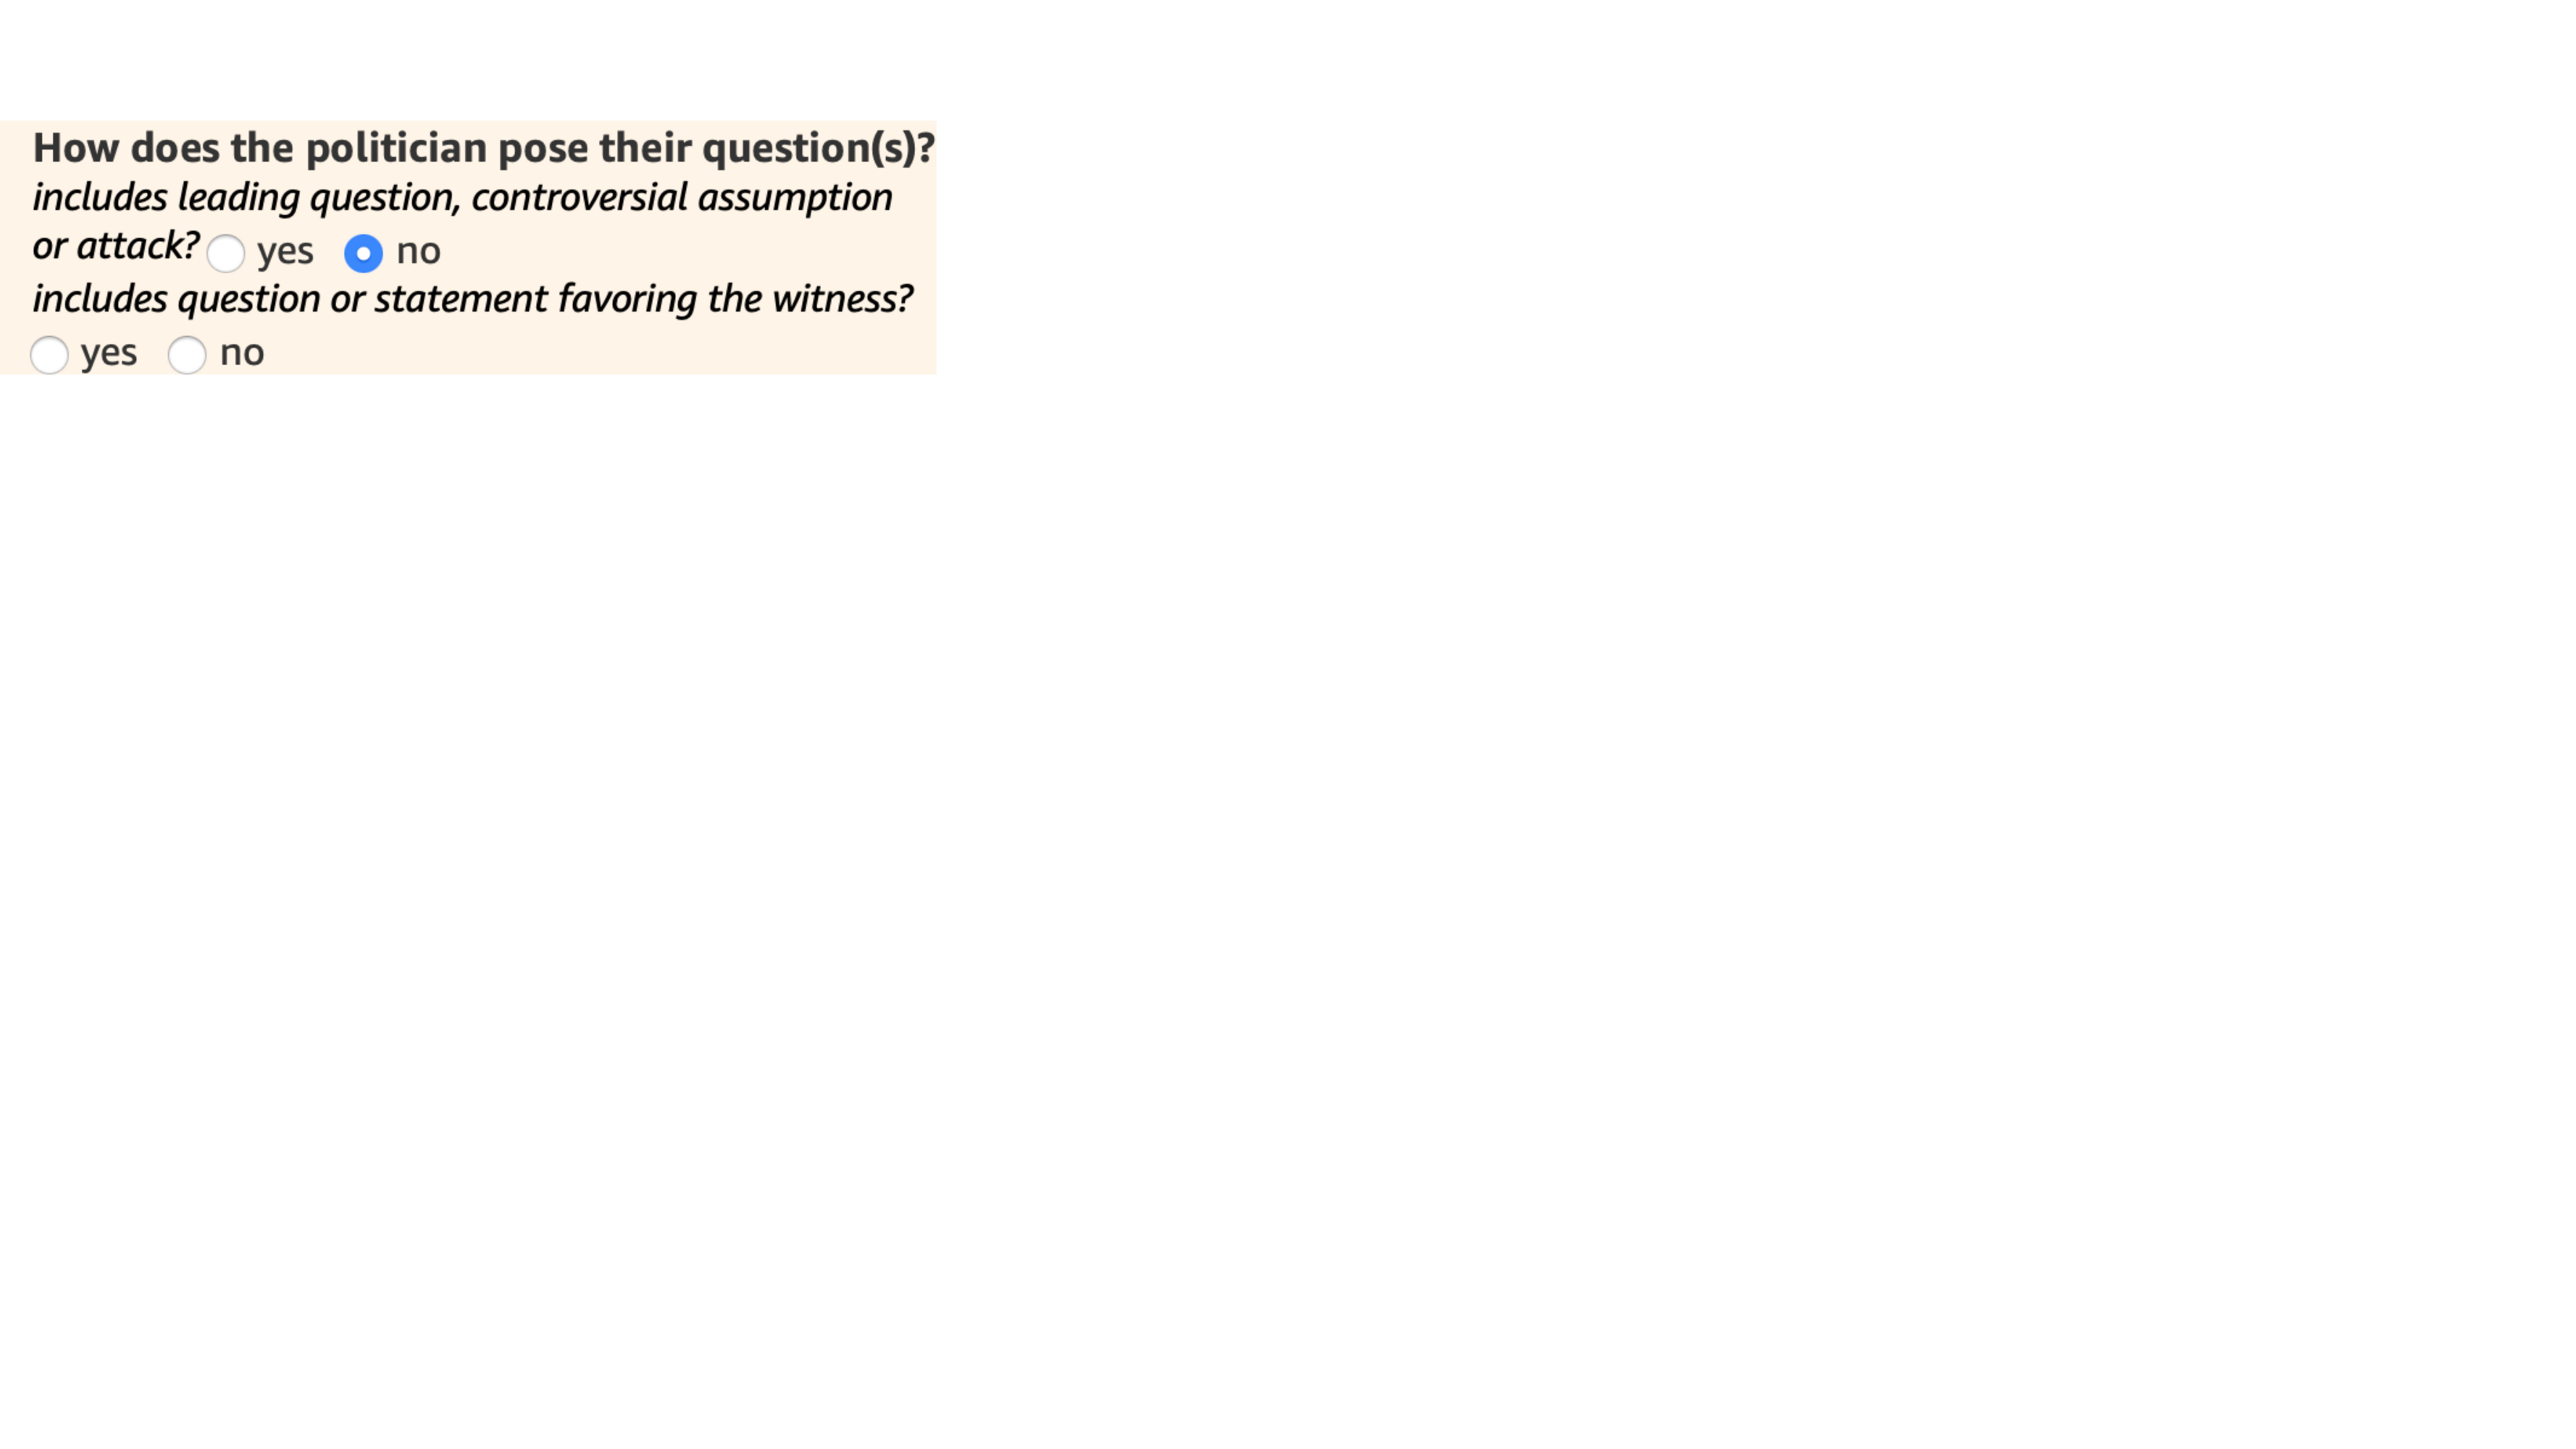
\includegraphics[width=1\linewidth]{plots/subj_amt_screenshots_question.pdf}
  \vspace{3.5em}
  \caption{question}
\end{subfigure}%
\begin{subfigure}{.45\textwidth}
  \centering
  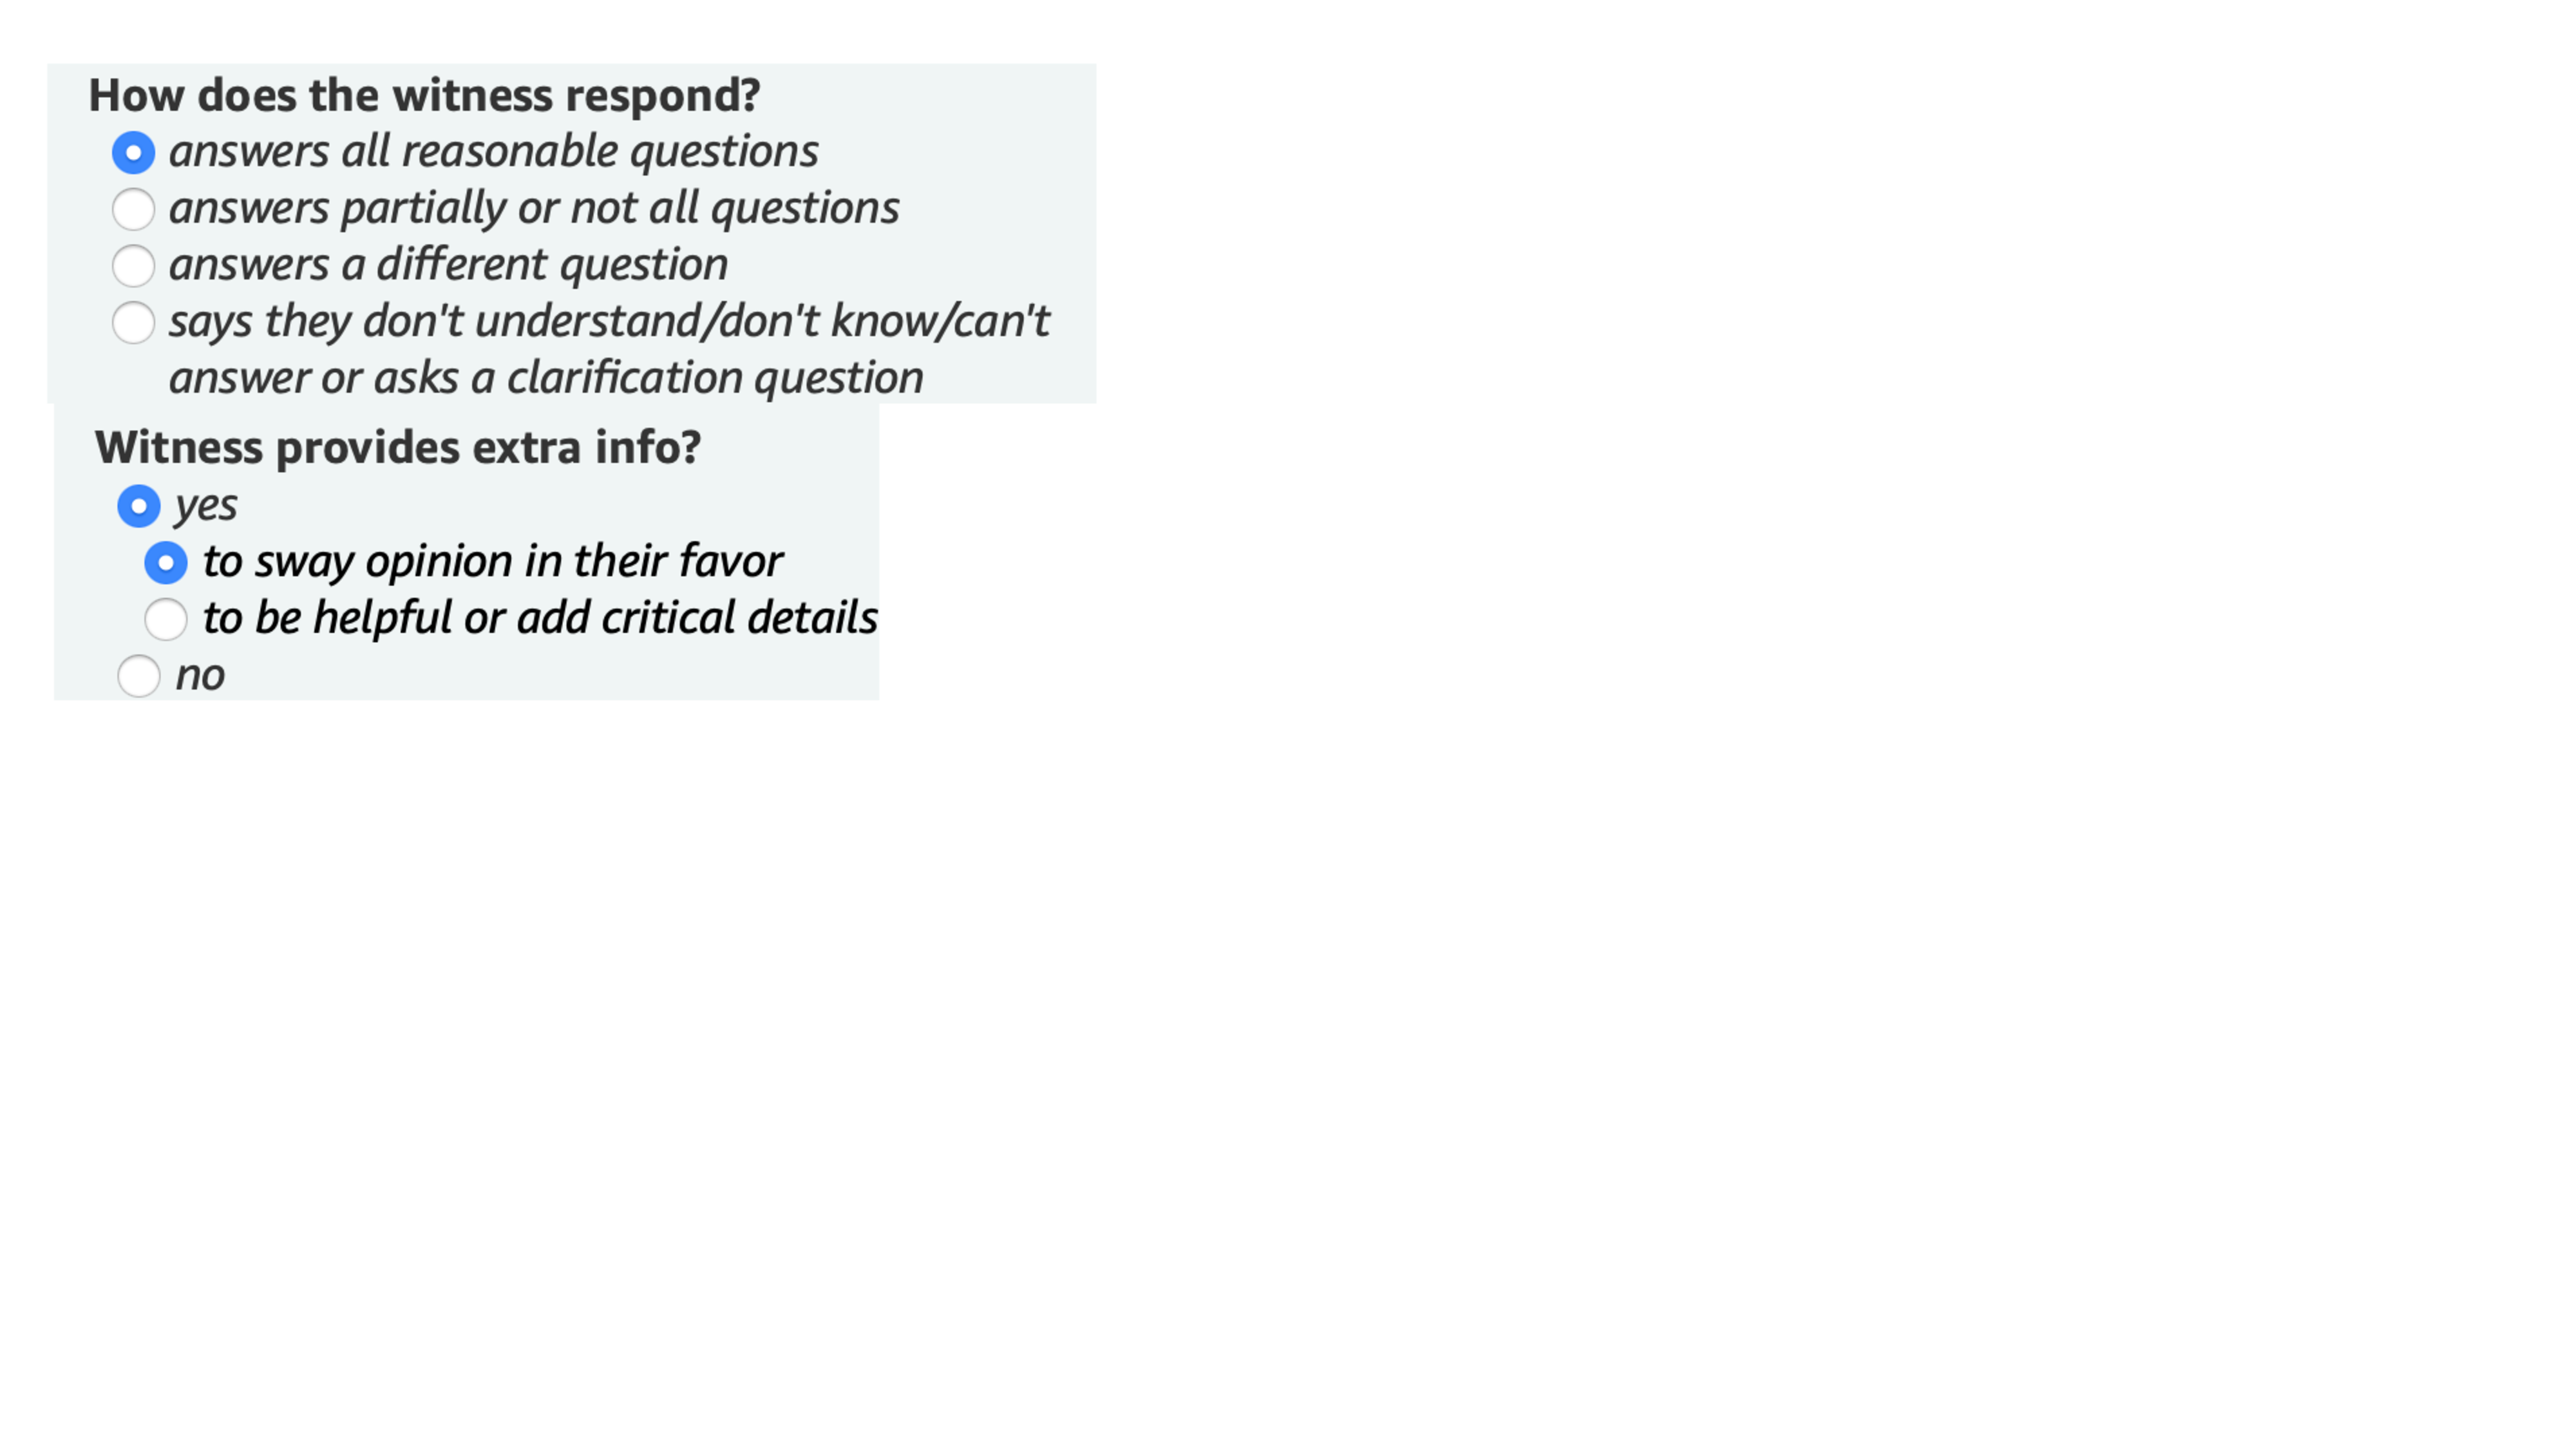
\includegraphics[width=1\linewidth]{plots/subj_amt_screenshots_overanswer.pdf}
  \caption{answer, overanswer}
\end{subfigure}\\
\begin{subfigure}{.34\textwidth}
  \centering
  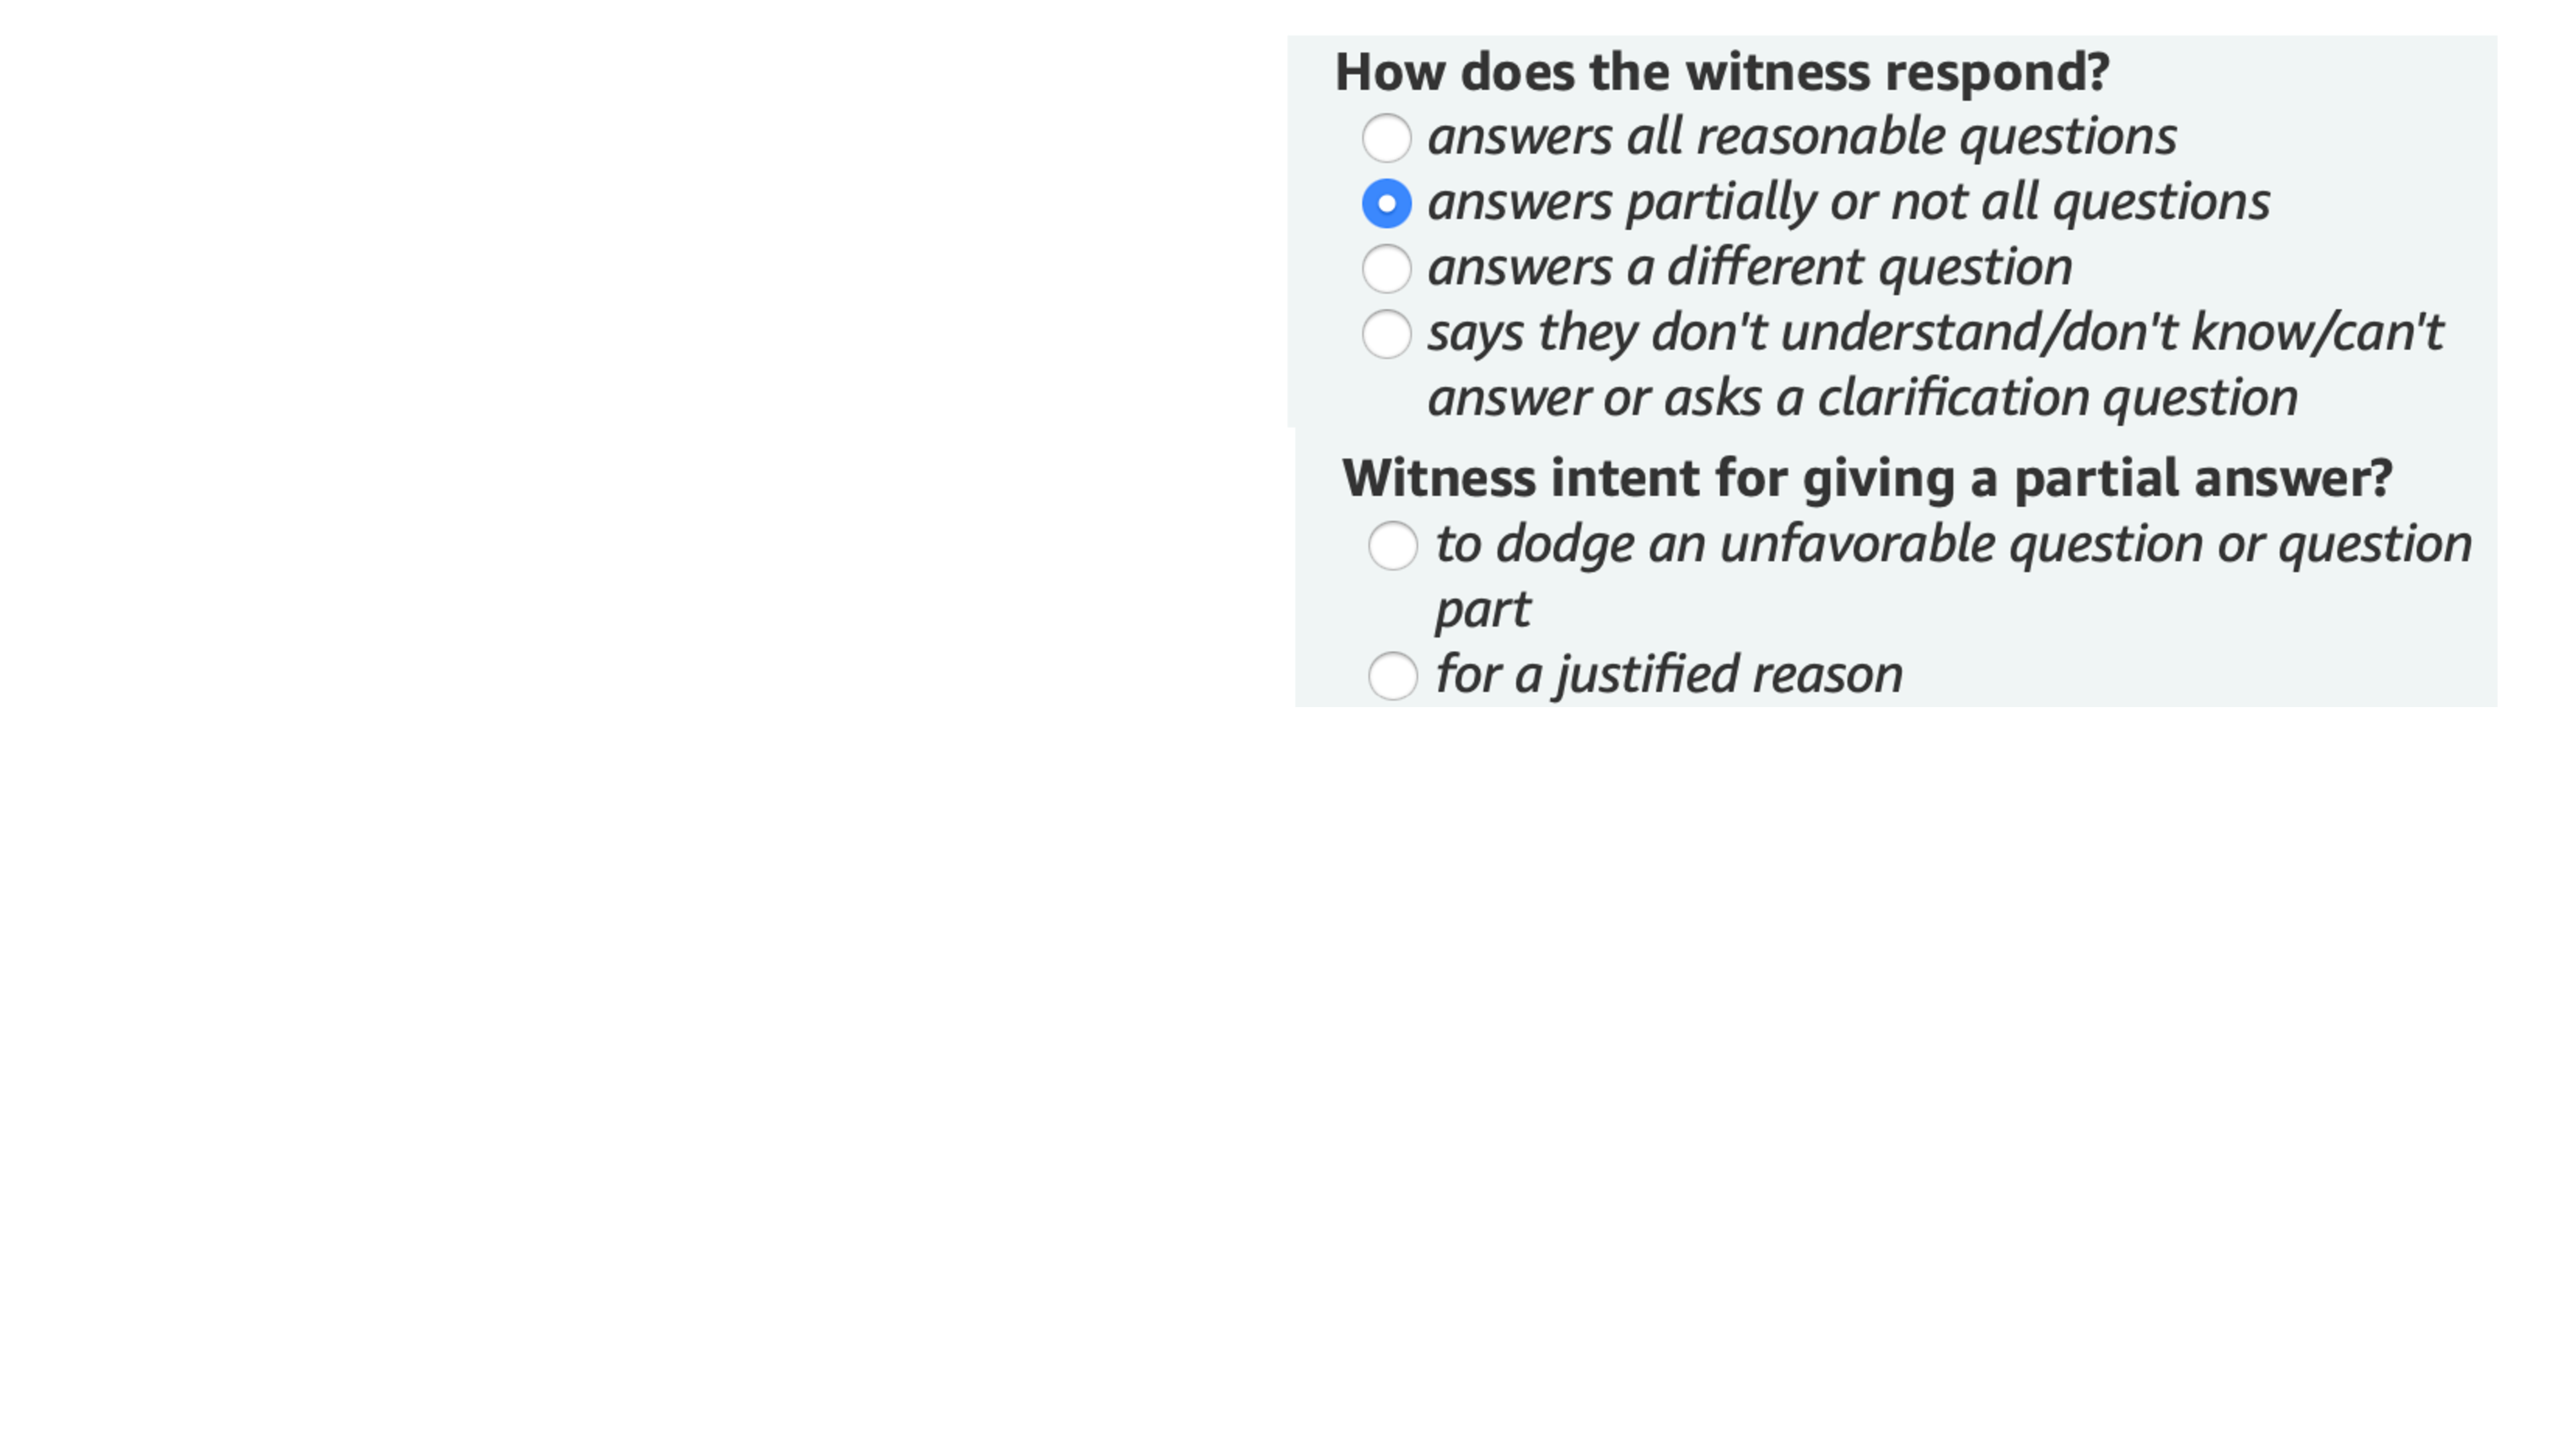
\includegraphics[width=1\linewidth]{plots/subj_amt_screenshots_response2.pdf}
  \vspace{0.003em}
  \caption{partial answer}
\end{subfigure}%
\begin{subfigure}{.34\textwidth}
  \centering
  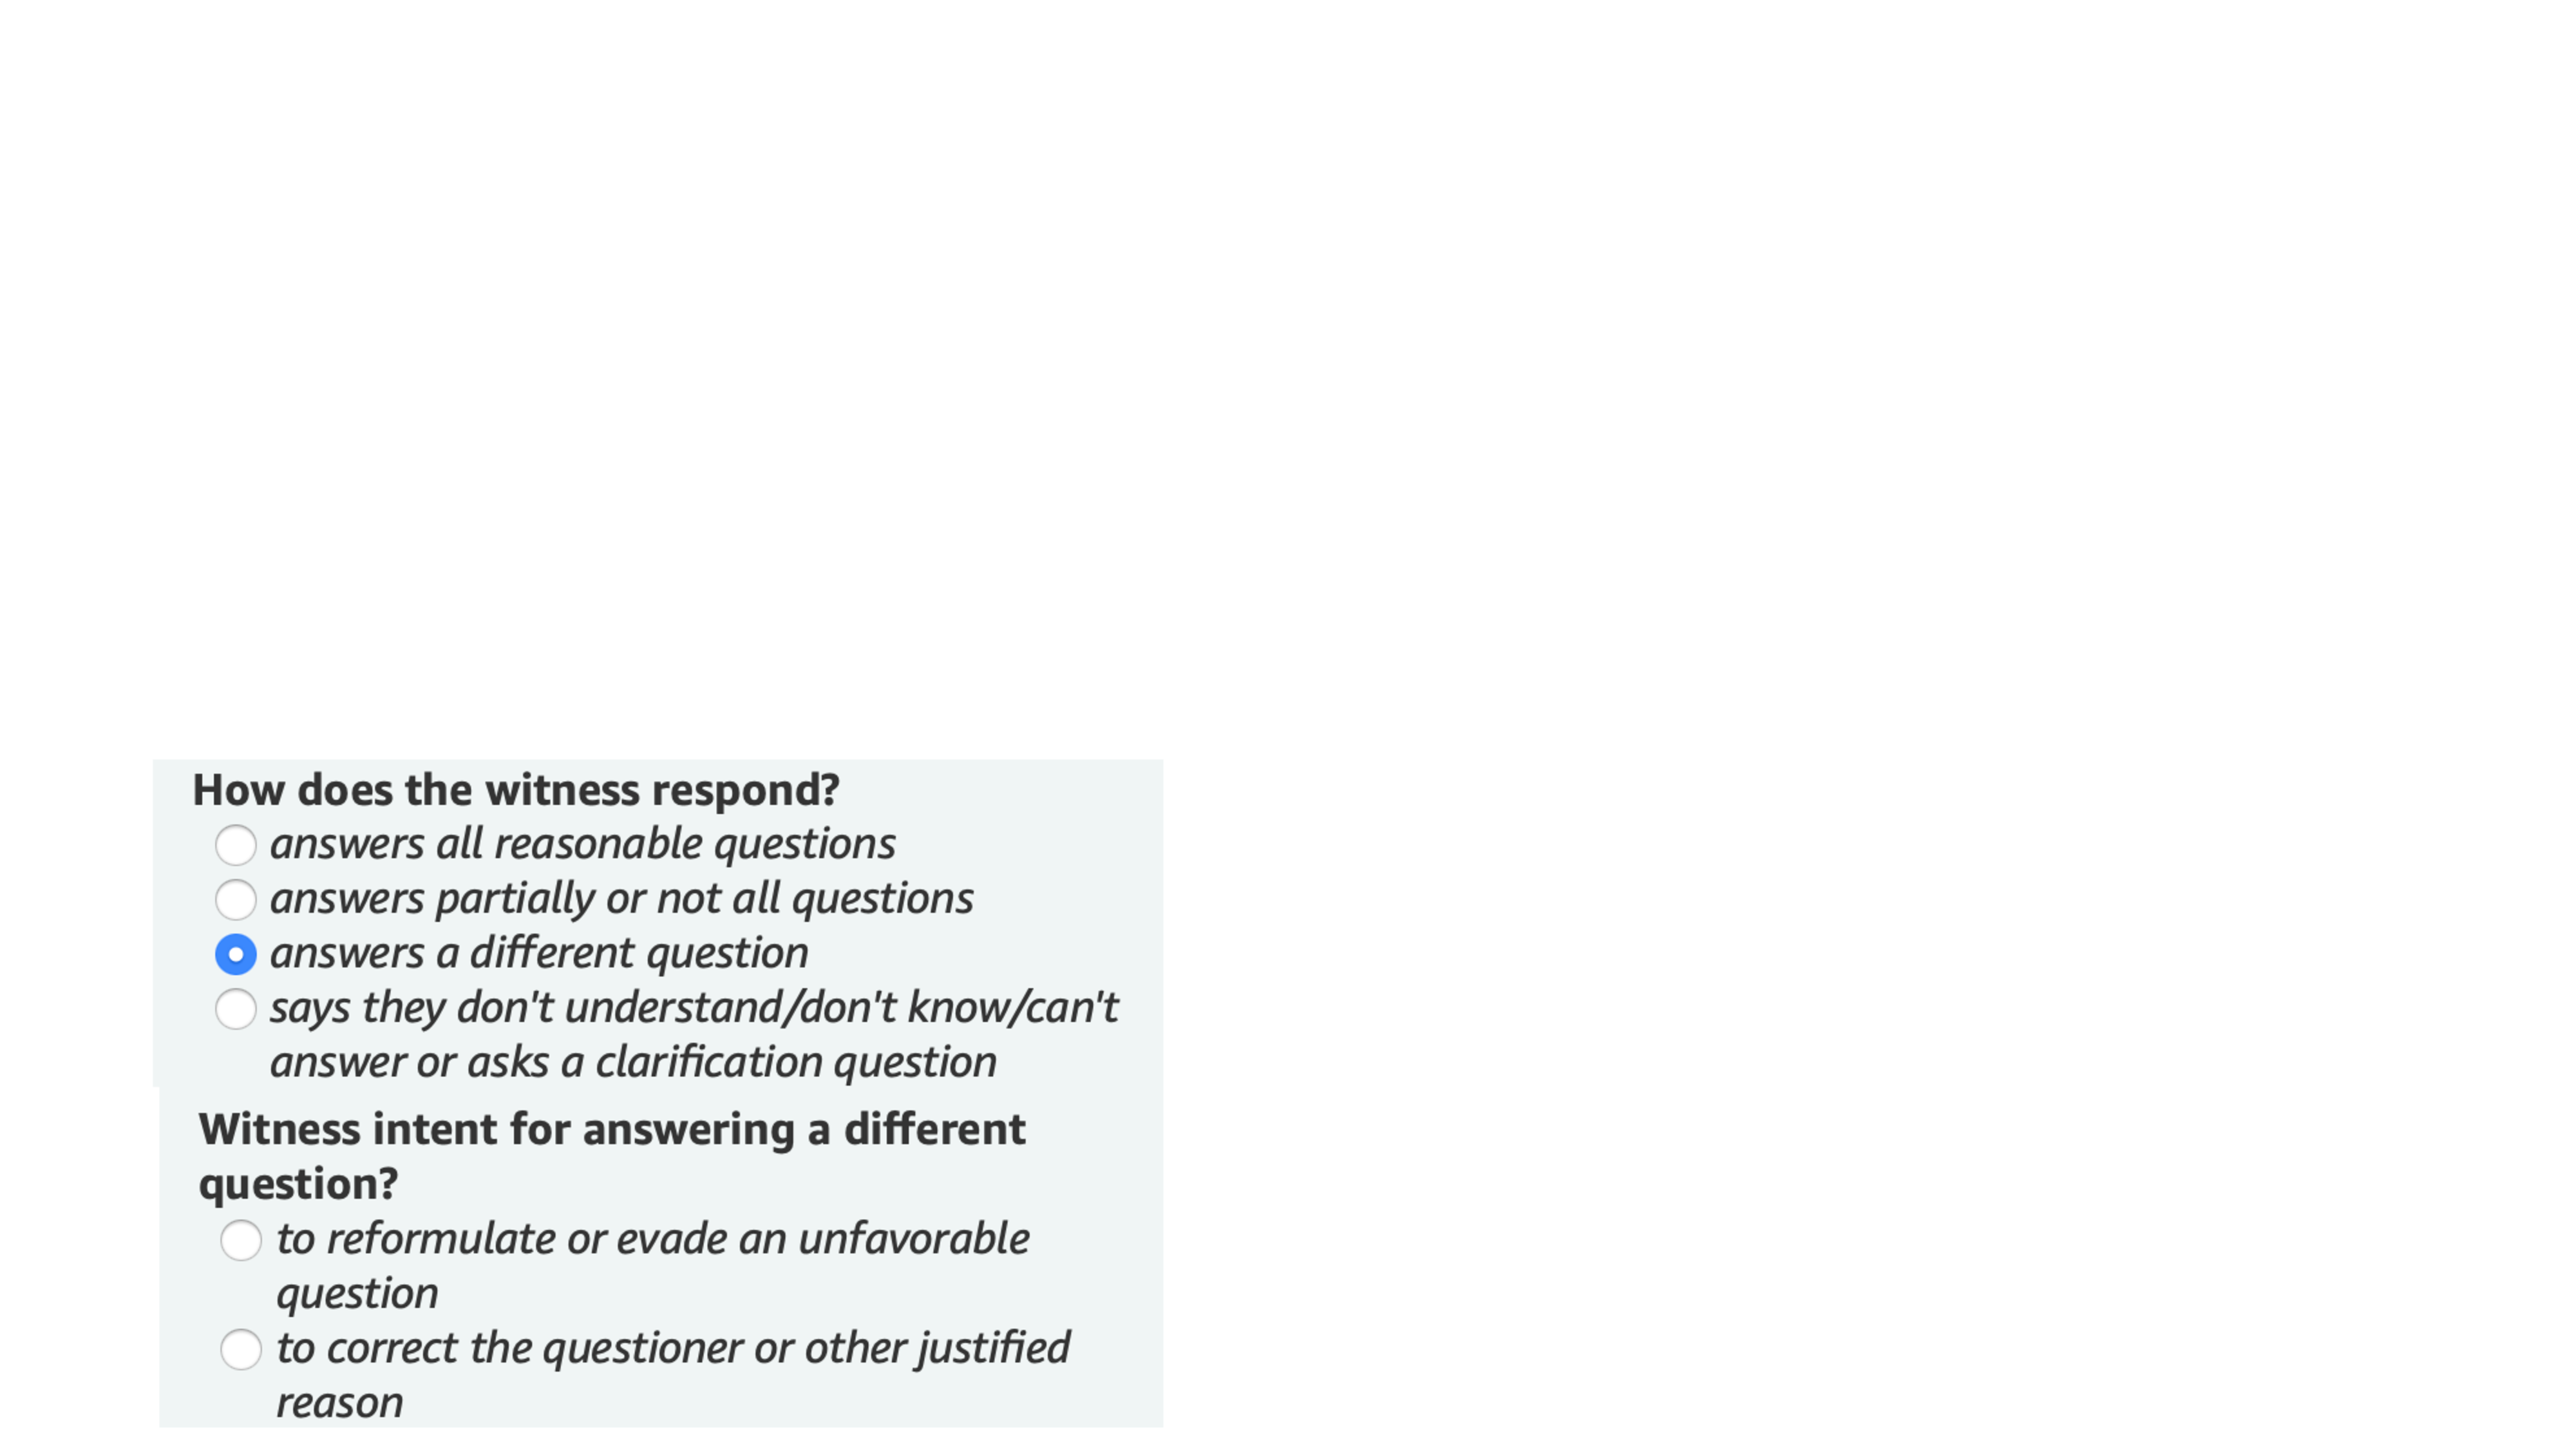
\includegraphics[width=1\linewidth]{plots/subj_amt_screenshots_response3.pdf}
  \caption{shifted answer}
\end{subfigure}%
\begin{subfigure}{.34\textwidth}
  \centering
  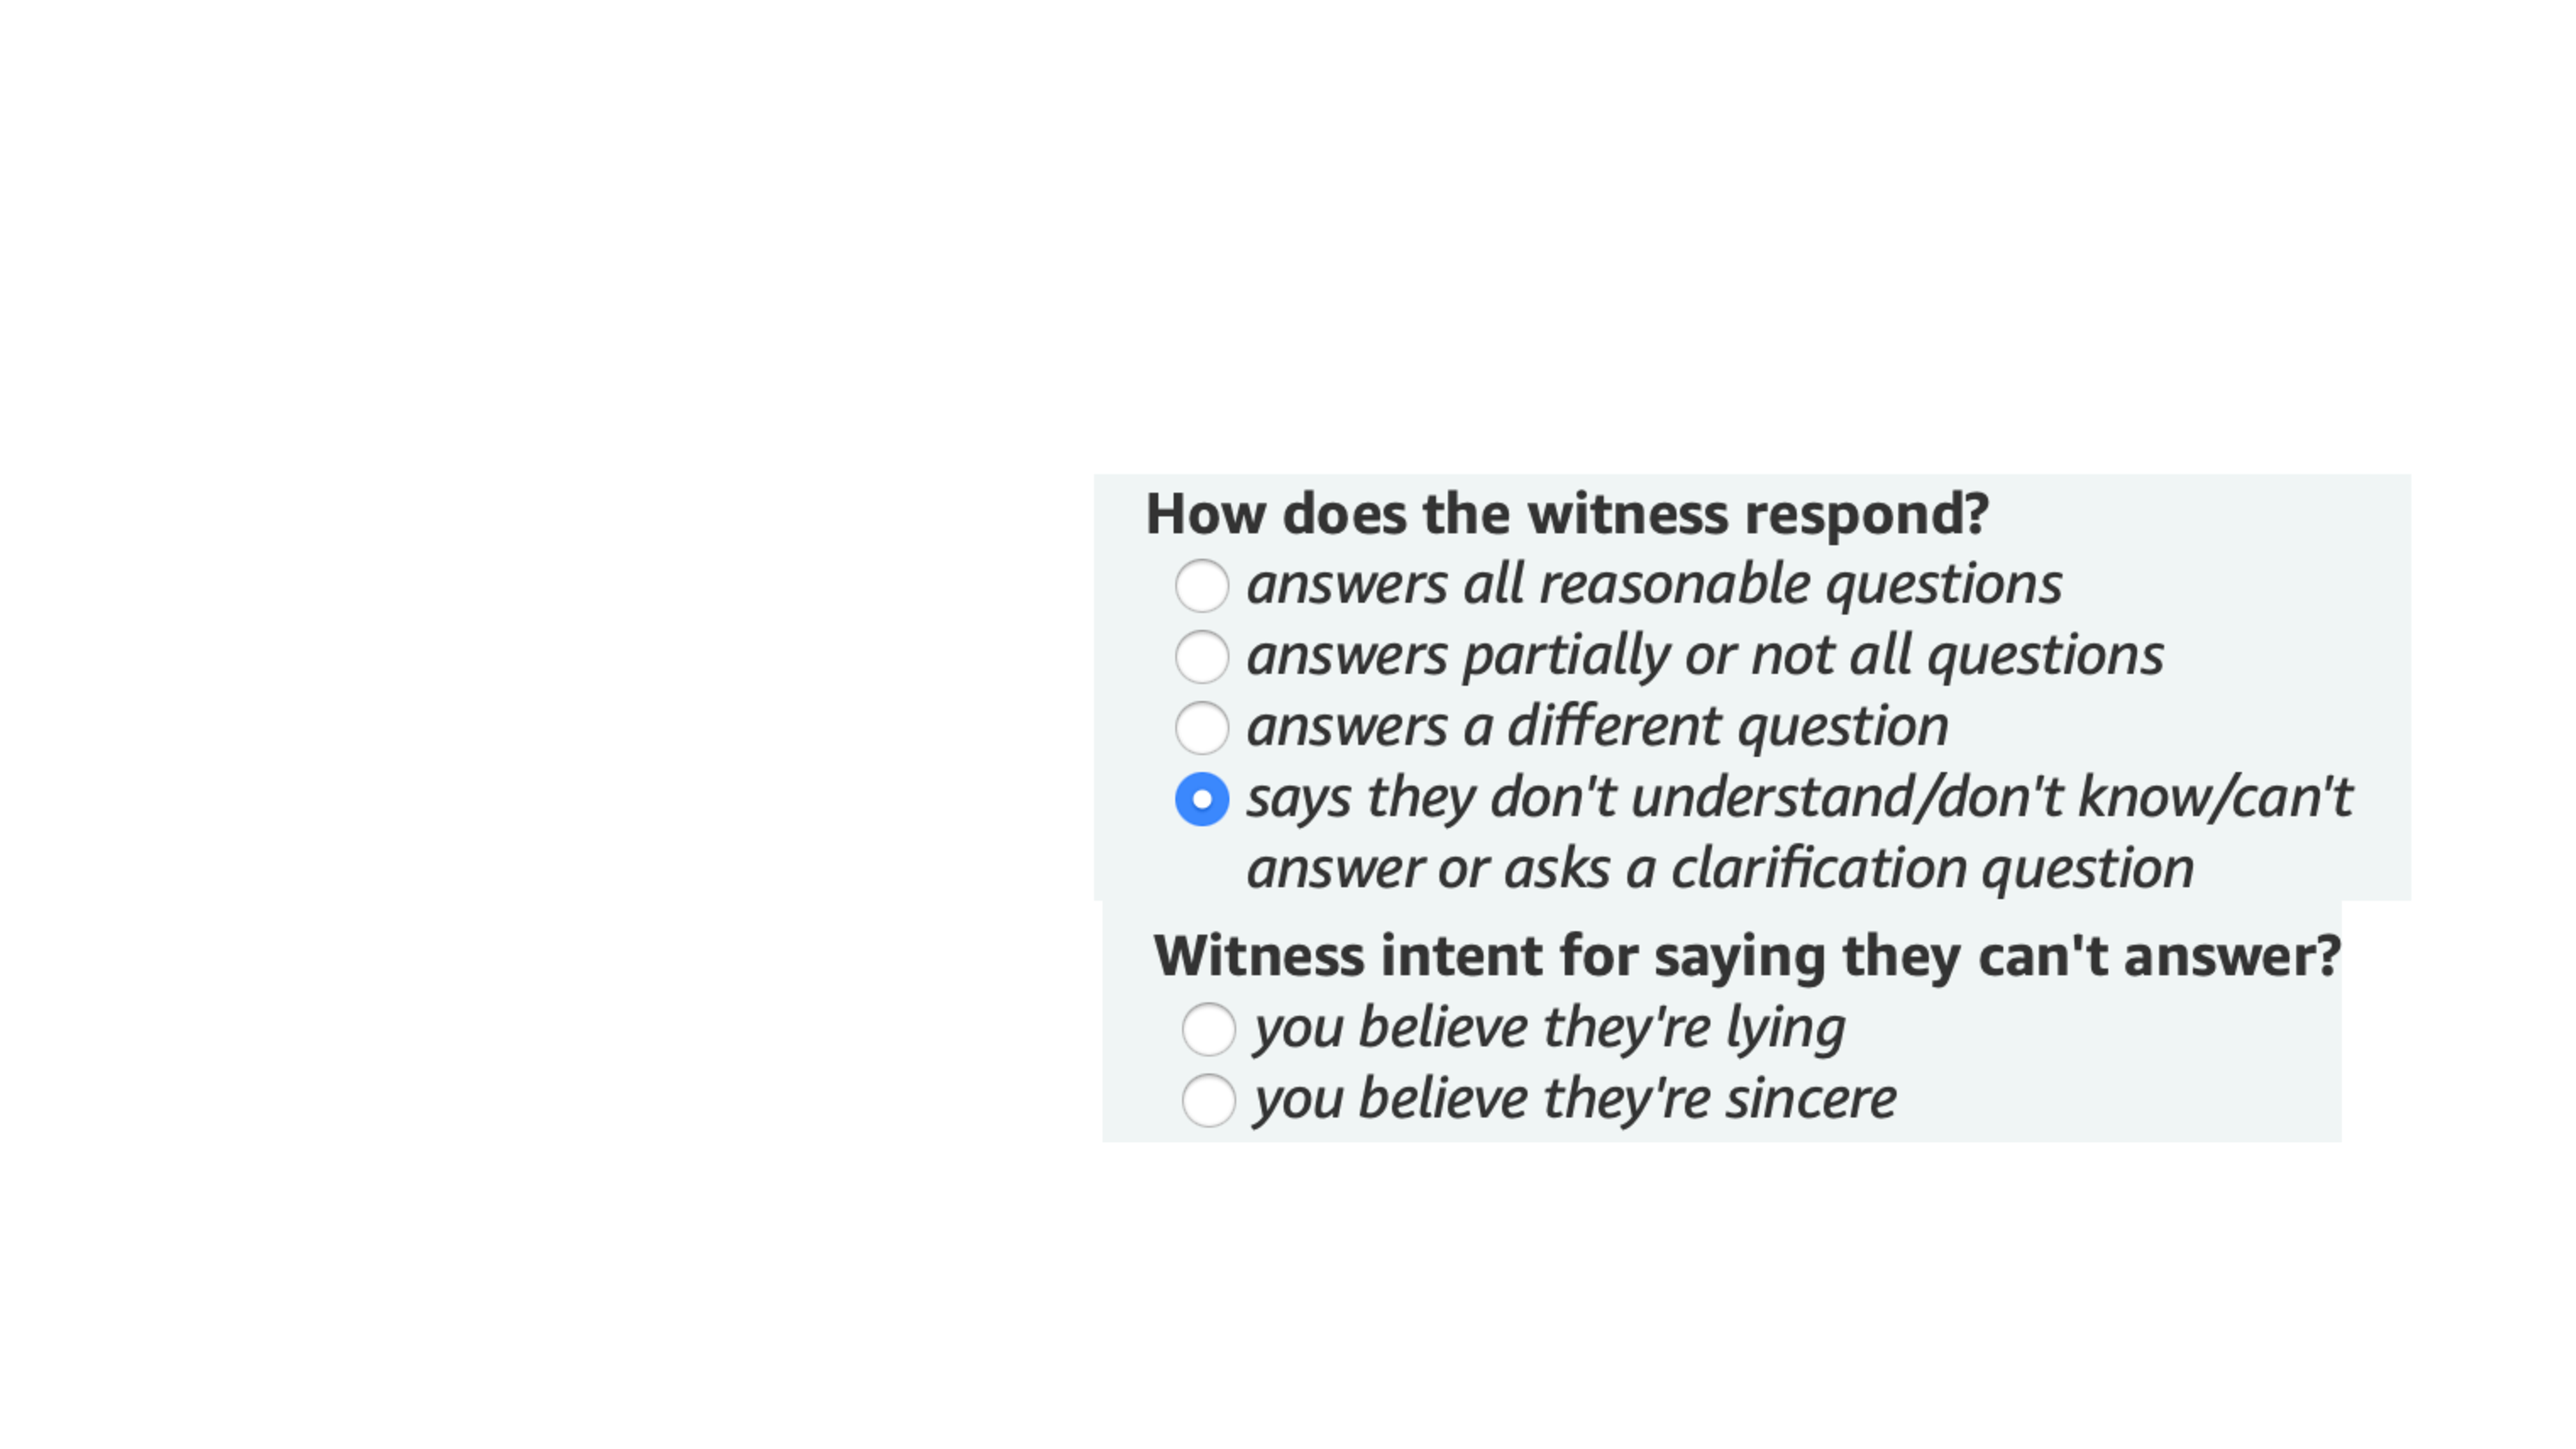
\includegraphics[width=1\linewidth]{plots/subj_amt_screenshots_response4.pdf}
  \vspace{.481em}
  \caption{can't answer}
\end{subfigure}
\caption{Nested questions that appear for the question (a) and for the response (b-e).}
\label{fig:subj_amt_screenshots_nested}
\end{figure}

\section{Annotator consistency}
\label{sec:app_consistency}
Due to an error creating annotation batches, 4 annotators were asked to annotate the same HIT twice. We take advantage of this fortuitous mistake to conduct a small-scale study of annotator consistency. Note that each annotator labeled a different HIT so we cannot compare between annotators. However, each HIT is the first of their hearing (that is, the first five question-response pairs), so all annotators were ostensibly encountering the witness and the hearing for the first time in their first annotation. We examine whether annotators change their labels for the question, the response or their sentiments towards the questioners and witness. We find the annotators are highly consistent in their sentiment towards the questioner (only 1 annotator changed while still having the same coarse-grained sentiment), and in their labels for the question and the response's conversation act (only 3/20 cases were changed for each label type). Annotators are slightly less consistent in their labels for the response intent (4/20 were changed). Interestingly, most of these intent changes (3 out of the 4) are from a positive to a negative intent and coincide with a change in annotator sentiment towards the witness also from positive to negative. This result leads us to the final finding that annotators are least consistent in their sentiment towards the witness (3/4 changed their sentiment to lean more negative, where 2/4 also had different coarse-grained sentiment). We speculate these results reflect a higher level of uncertainty towards the witness at the beginning of a hearing (where annotators err on the positive side, assuming a cooperative witness) which can then resolve itself as more of the hearing is presented to the annotator. 

\section{Training details}
\label{sec:app_training}

All models are trained on an NVIDIA Quadro RTX 6000 GPU. For hyperparameter tuning, we use early stopping based on development macro-F1 with a patience of 10 epochs and average results across 3 runs with different random initializations. For test, we train for 30 epochs and then evaluate on the test fold. If training does not improve by 40\% in the first 15 epochs, then training is restarted. We repeat this process for each test set across the 4 folds.

For the \textsc{RoBERTa} classification task and all models that build on top of it, we use a learning rate of 1e-5, a warmup proportion of 0.01, no weight decay and batch size of 8, max sequence length of 512. For the \textsc{RoBERTa} regression task, we use a learning rate of 5e-5, a warmup proportion of 0.1 and weight decay of 0.01 (batch size and max sequence length are unchanged).

\section{Model variants}
\label{sec:app_variants}

In Table \ref{tab:other_models} include results with additional baselines, pretrained language models and adding other forms of context to the \textsc{Hierarchical} model.

\begin{table}[t]
\centering
\small
\begin{tabular}{ll}
\toprule
Model & macros-F1\\
\midrule
Regularized LSTM &42.98 (0.07) \\
Hierarchical Attention Network &43.05 (0.12)\\
\midrule
ALBERT &55.88 (0.08)\\
ELECTRA &55.83 (0.05)\\
\midrule
+Entire Question &52.37 (0.36)\\
+Last Interrogative Sentence &55.75 (0.28) \\
+Question Intents &58.66 (0.11)\\
+Fine-grained Witness Sentiment &59.70 (0.03)\\
+Fine-grained Questioner Sentiment &56.41 (0.27)\\
+Coarse-grained Questioner Sentiment &56.61 (0.28)\\
\bottomrule
\end{tabular}
\caption{Results on additional baselines (top), pretrained language models (middle), and incorporating other contexts.}
\label{tab:other_models}
\end{table}

\section{Additional dataset analyses}
\label{sec:app_lmi}

\begin{table}[t]
\centering
\small
\begin{tabular}{ll}
\toprule
label  & top LMI ngrams\\ 
\midrule
\texttt{ans+direct}  &`yes', `be correct'  \\
\texttt{ans+overanswer} &`think', `think that' \\
\texttt{shift+dodge} &`we', `--'\\
\texttt{shift+correct} &'--', `be something'\\
\texttt{cant\_ans+lying} &'I', '?', 'not'\\
\texttt{cant\_ans+sincere} &'I', 'not', '?'\\
\bottomrule
\end{tabular}
\caption{Ngrams with highest LMI scores for each label.}
\label{tab:subj_lmi}
\end{table}

In order to assess whether our dataset has annotation artifacts that would allow a model to easily `cheat' by focusing only on lexical cues (a more common effect in annotator-generated data, such as inserting a negation to generate a contradiction in Natural Language Inference \cite{Gururangan:2018}), we follow the approach in \newcite{Schuster:2019} to conduct an analysis of the local mutual information (LMI) between the labels and the response text unigrams, bigrams and trigrams. Unlike pointwise mutual information, LMI highlights \emph{high frequency} words that co-occur with the label. We summarize our results in Table \ref{tab:subj_lmi}, finding most labels have a meaningful cue. The \texttt{ans+direct} cues signal a straight answer. The dashes for both \texttt{shift} labels are usually an indicator the witness was interrupted (recall this label includes partial answers). Interestingly, both \texttt{cant\_answer} labels have the same cues, which include negation (to indicate not being able to answer) and a question mark for clarification questions. We expect these cues to possibly help with conversation act identification, but less so with intent.
